\section{Road Generation}

After the city markers are specified and the population density map has been created, it is time to generate the road network.
Using the markers, the road generator creates workers called Agents in the area specified by the markers and assigns them strategies depending on the corresponding city type.
The purpose of the strategies is solely to give Agents instructions for movement and termination.
Strategies take a few different variables into account when it decides these actions, for example the amount of steps an Agent has taken so far, the population density, and if the Agent has landed on an existing road.
The application has Agent strategies for Paris and Manhattan cities, and an example of these are shown in Figure~\ref{fig:results_city_paris} and Figure~\ref{fig:results_city_manhattan}.

How the roads are created and connected is entirely up to the road network.
It handles placing down road nodes and connecting them together, making sure that intersections are created where necessary.
The Agents simply instruct the road network where it wants to place down roads, and the network handles the rest while also providing the Agent with information of how the road network was modified.
Then, the strategies can use that information and react accordingly, for example to terminate the Agent.

From Figure~\ref{fig:results_real_city_manhattan} we can clearly observe the distinct grid-like structure of the road network, which in turn was the goal for our Manhattan generation strategy.
The overall shape of the city does not necessarily mimic the shape of Manhattan in the real world because Manhattan is surrounded by water, something that we are not required to have in our application.
If the city marker is placed on an isolated island, it would be much closer to the aspects of Manhattan in the real world.

\begin{figure}[H]
  \centering
  % Use two minipages to add padding for the figure and its caption
  \begin{minipage}{.45\textwidth}
    \centering
    \begin{minipage}{.9\textwidth}
      \centering
      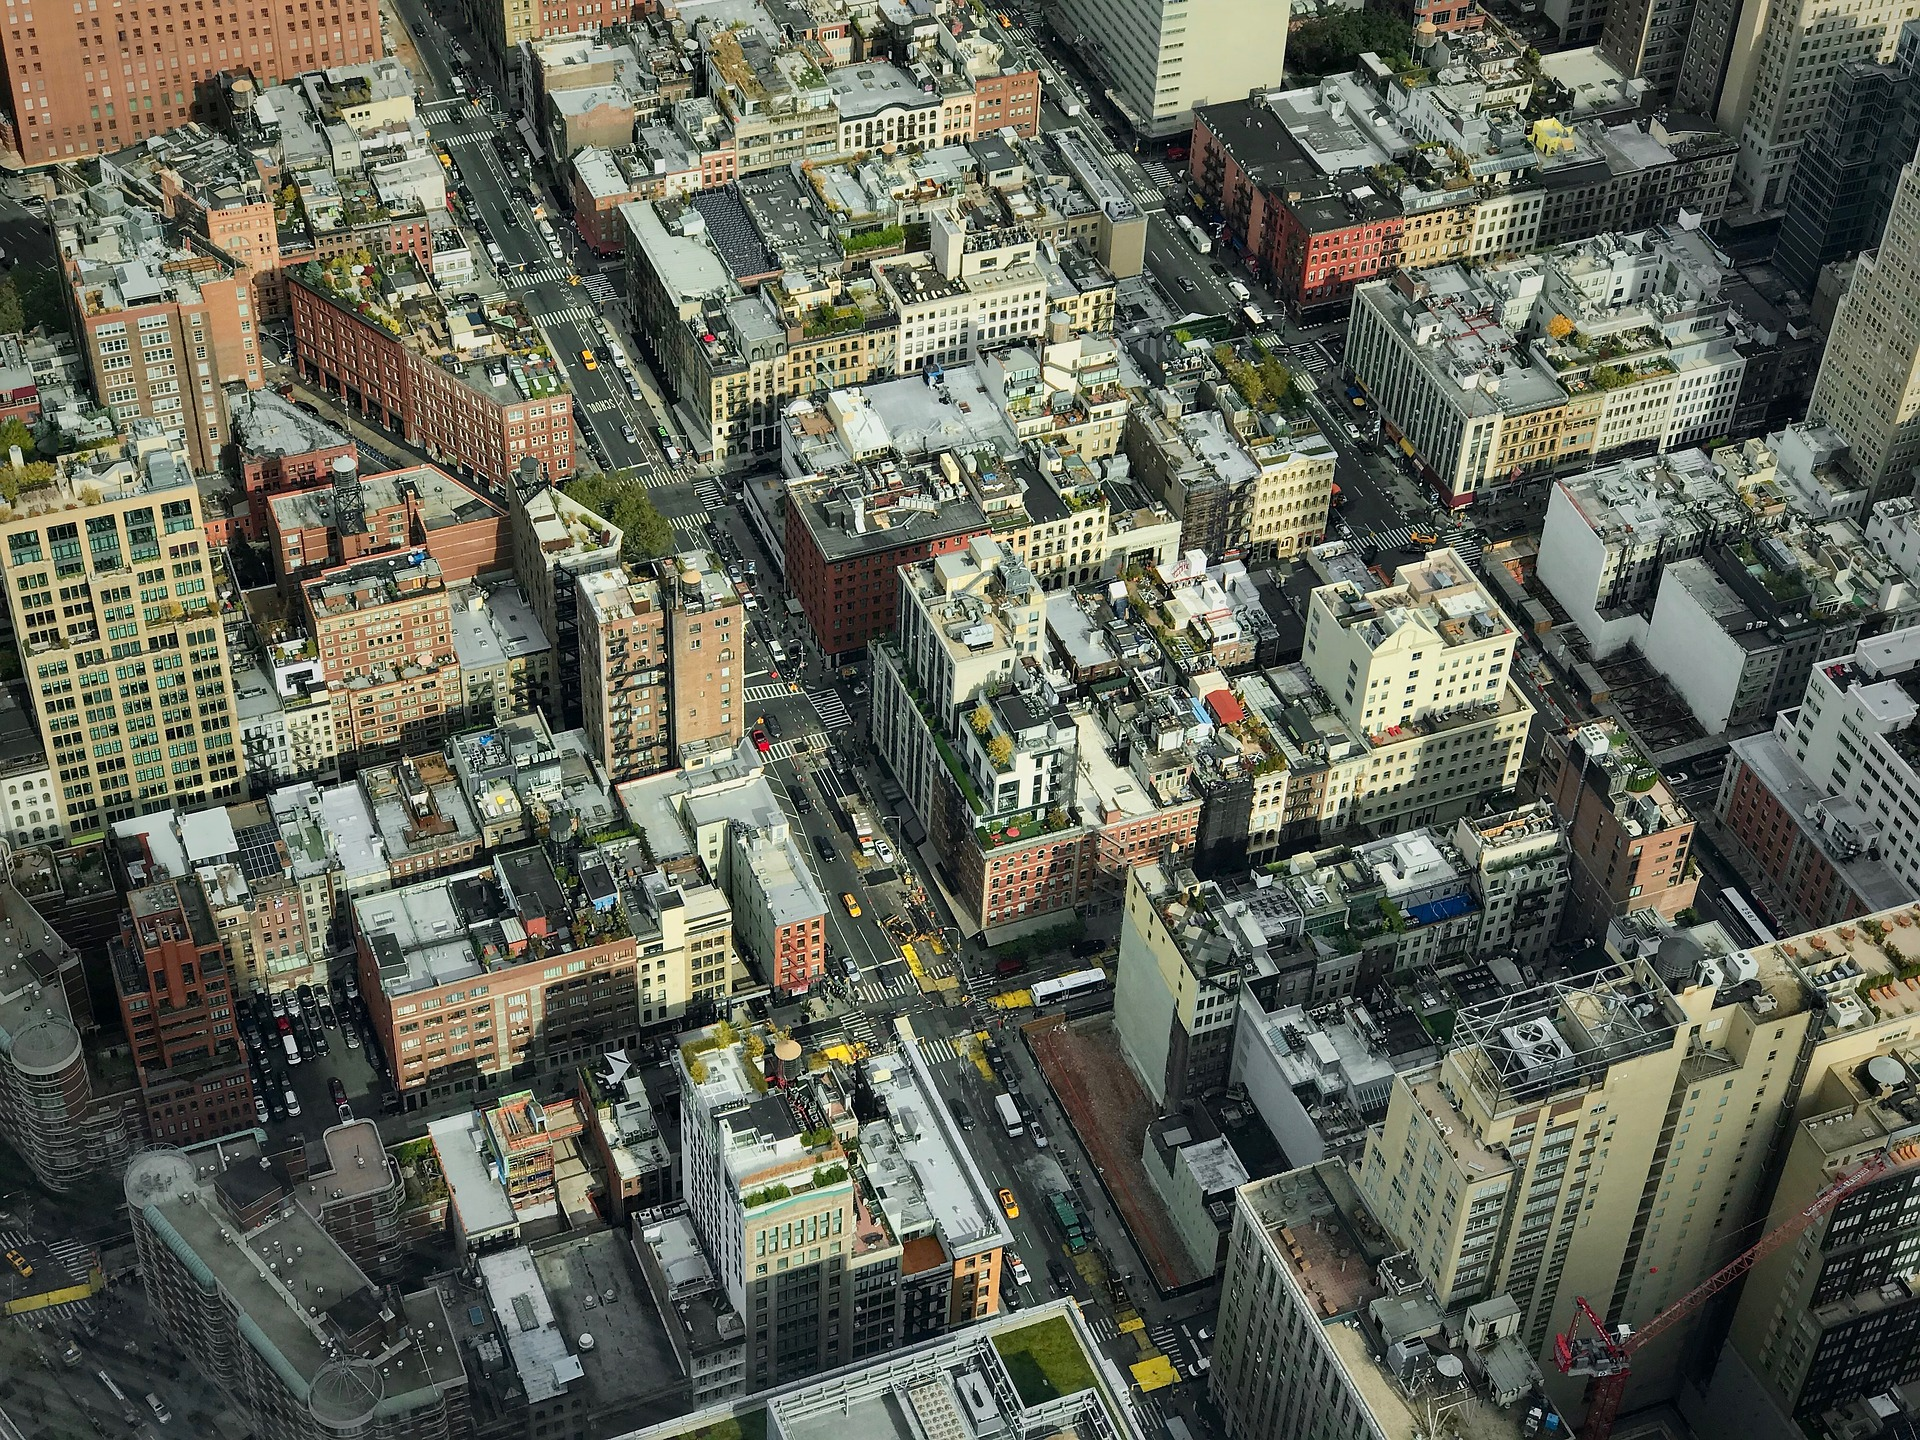
\includegraphics[width=\textwidth]{figure/results/manhattan.jpg}
      \caption{Picture of Manhattan grid-like road system~\cite{manhattan_city_img}.}
      \label{fig:results_real_city_manhattan}
    \end{minipage}
  \end{minipage}
  \begin{minipage}{.45\textwidth}
    \begin{minipage}{.9\textwidth}
      \centering
      \centering
      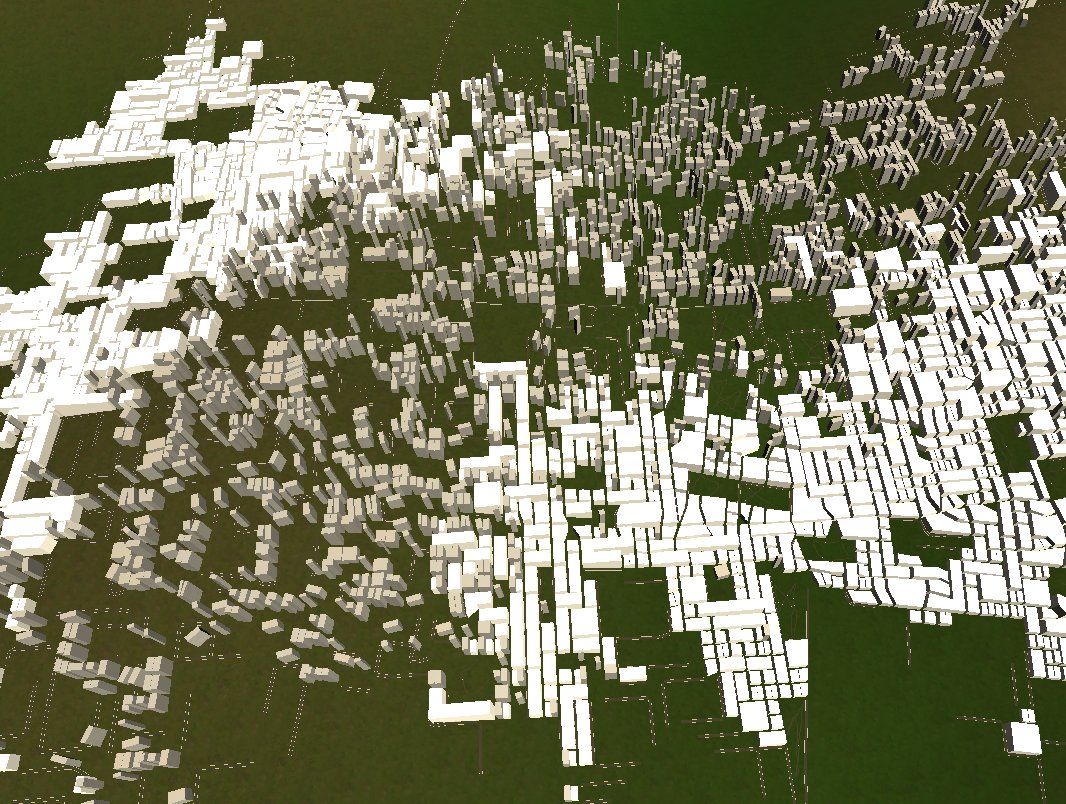
\includegraphics[width=\textwidth]{figure/results/city_manhattan.png}
      \caption{Example of a fully generated Manhattan-style city.}
      \label{fig:results_city_manhattan}
    \end{minipage}
  \end{minipage}
\end{figure}

Meanwhile, Paris has a very different overall aesthetic than Manhattan.
Around the Arch de Triomphe in Figure~\ref{fig:results_real_city_paris}, there are distinct rings and roads extending from the center, which is something we aimed to mimic in this project.
In the generated city in Figure~\ref{fig:results_city_paris}, the structure does have distinct rings and roads similar to the pattern in Paris. 

\begin{figure}[H]
  \centering
  % Use two minipages to add padding for the figure and its caption
  \begin{minipage}{.45\textwidth}
    \centering
    \begin{minipage}{.9\textwidth}
      \centering
      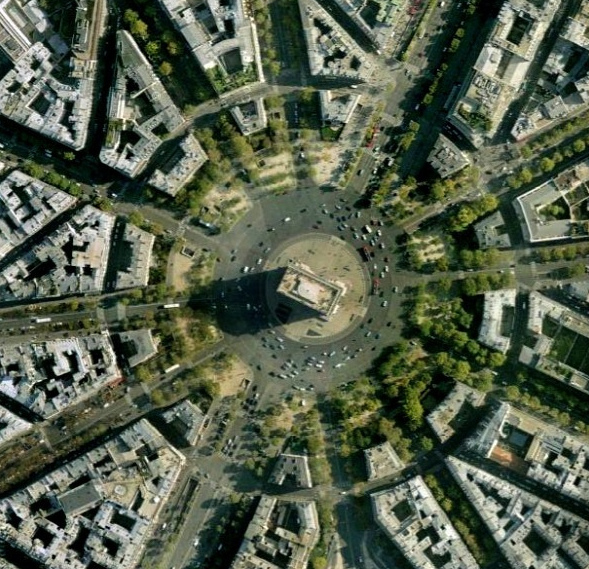
\includegraphics[width=\textwidth]{figure/results/paris_arc_de_triomphe.jpg}
      \caption{Picture of Paris ring-like road system~\cite{paris_city_img}.}
      \label{fig:results_real_city_paris}
    \end{minipage}
  \end{minipage}
  \begin{minipage}{.45\textwidth}
    \begin{minipage}{.9\textwidth}
      \centering
      \centering
      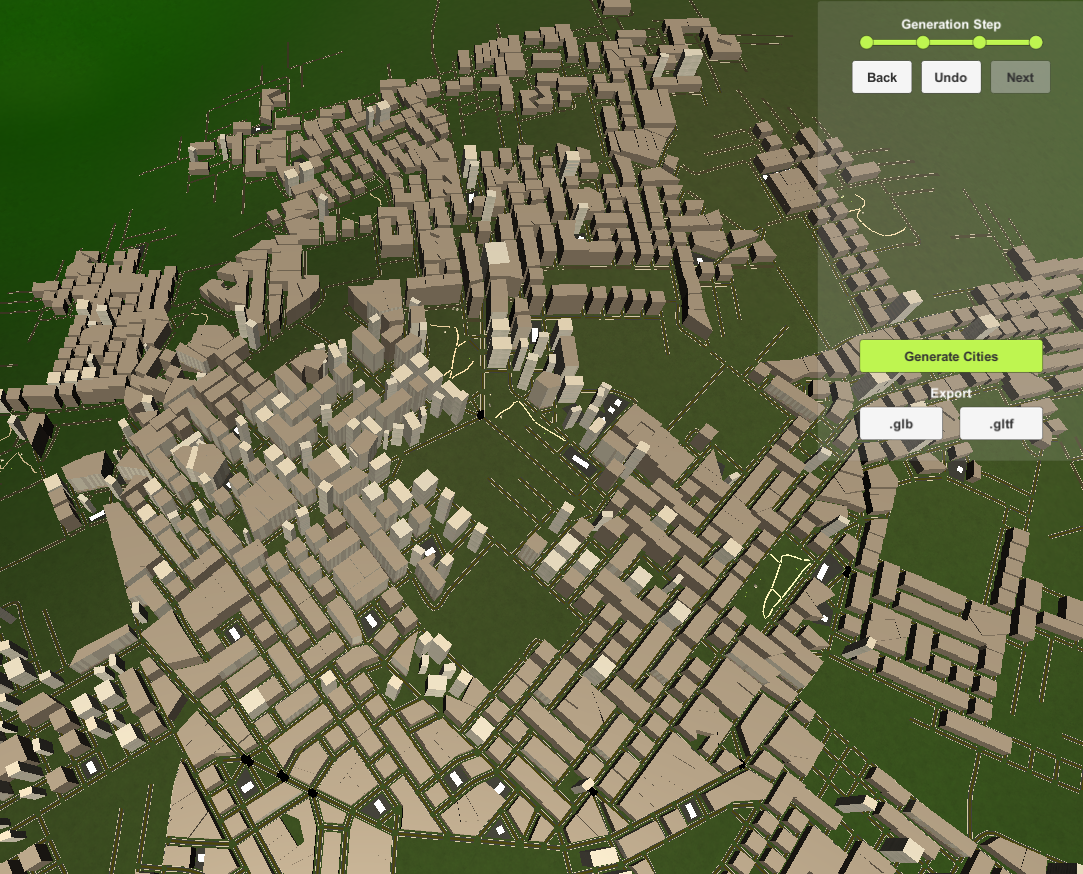
\includegraphics[width=\textwidth]{figure/results/city_paris.png}
      \caption{Example of a fully generated Paris-style city.}
      \label{fig:results_city_paris}
    \end{minipage}
  \end{minipage}
\end{figure}

Both city types have streets branching out from their main roads, which in turn also branch out from themselves to form a grid-like street neighborhood.
These streets are created using a street strategy which is shared between the strategies used for the two different city types, however it is possible to implement more complex street strategies for other types of cities.

When Agents travel too far away from the city boundaries, which are defined by the city markers in the beginning of the generation, they switch to a highway strategy.
The purpose of the highway strategy is simply to create longer roads with little change in direction.
It also aims to follow the population map density to some degree, especially navigating towards higher populated areas.
This results in highways which typically connect cities together.
